\documentclass[xcolor={table}]{beamer}
\usetheme{Singapore}
\usepackage[utf8]{inputenc}
\usecolortheme{crane}
\usepackage{graphicx}
\usepackage{standalone}
\usepackage{tikz}
\usetikzlibrary{arrows}
\usetikzlibrary{decorations.markings}
\usetikzlibrary{calc}
\usetikzlibrary{shapes,snakes}
\usepackage{amsmath}
\usepackage{amsfonts}
\usepackage{amsthm}
\usepackage{mathtools}
\usepackage{tcolorbox}

\definecolor{lightblue}{RGB}{124,190,255}
\definecolor{darkgreen}{RGB}{24,145,0}
\definecolor{textorange}{HTML}{cc5200}

\beamertemplatenavigationsymbolsempty
\setbeamerfont{caption}{size=\tiny}

\title{$3^{\text{rd}}$ Year Writing Workshop}
\author{}
\date{}

\begin{document}

\maketitle

\begin{frame}
\begin{quote}\Large
``If you want to be a writer, you must do two things above all others: read a lot and write a lot.''\\
\hfill Stephen King
\end{quote}
\end{frame}

\begin{frame}
\frametitle{Reading}
Read the two pieces of mathematical writing.

Consider:
\begin{itemize}
  \item the audience
  \item the style
  \item the message
  \item how effective it is in communicating that message
  \item any gaps / unanswered questions
  \item likes \& dislikes
\end{itemize}
\end{frame}


\begin{frame}
\frametitle{Some Guidelines (Francis Edward Su)}
\centering
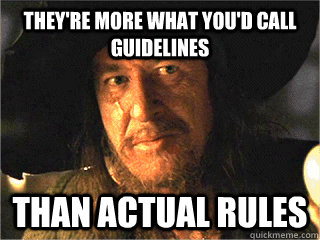
\includegraphics[width=0.8\textwidth]{../img/guidelines.jpeg}
\end{frame}

\begin{frame}
\frametitle{Some Guidelines (Francis Edward Su)}
\begin{columns}
\begin{column}{0.44\textwidth}
\begin{enumerate}
  \item<1-> Know your audience.
  \item<2-> Friendly tone.
  \item<3-> Write in sentences.
  \item<6-> Be picky.
  \item<7-> Use and highlight structure.
  \item<8-> Refine and simplify.
\end{enumerate}
\end{column}
\begin{column}{0.56\textwidth}
\scriptsize
\begin{tcolorbox}[colback=textorange!20, colframe=textorange, height=6.5cm, valign=center, right=1mm, left=1mm]
\only<1>{
  \begin{itemize}
    \item School children
    \item General public
    \item General scientists
    \item Mathematicians not in your field
    \item Mathematicians in your field
    \item Collaborators
    \item Yourself
    \item Your supervisor
    \item Your examiner
  \end{itemize}
}
\only<2>{
  \textbf{DOs}
  \begin{itemize}
  	\item Present tense
  	\item Inclusive pronouns: ``We construct...''
  	\item Guide the reader: ``Recall that...''
  \end{itemize}
  \vspace{5mm}
  \textbf{DON'Ts}
  \begin{itemize}
  	\item Confuse / intimidate
  	\item Patronise: ``It's obvious that...''
  	\item Belittle: ``...some basic algebra...''
  \end{itemize}
}
\only<3>{
\begin{columns}
\tiny
\begin{column}{0.25\columnwidth}
\begin{align*}
f(x) = g(x)\\
x^2 = x + 6\\
x^2 - x - 6 = 0\\
(x - 3)(x + 2) = 0\\
x = 3, \; x = -2
\end{align*}
\end{column}
\hspace{-20pt}
\vrule{}
\hspace{5pt}
\begin{column}{0.55\columnwidth}
The points where $f(x) = x^2$ and $g(x) = x + 6$ intersect are those that solve the equation defined by the functions being equal, that is
\begin{equation*}
x^2 = x + 6.
\end{equation*}
Rearranging this equation gives the following quadratic
\begin{equation*}
x^2 - x - 6 = 0,
\end{equation*}
and factorising this gives:
\begin{equation*}
(x - 3)(x + 2) = 0
\end{equation*}
which is satisfied when $x = 3$ or when $x = -2$.
\end{column}
\end{columns}
}
\only<4>{
Consider ``$A = 5$'':

\vspace{5mm}

Does this mean:
\begin{itemize}
  \item ``Let $A = 5$''?
  \item ``Suppose $A = 5$''?
  \item ``Therefore $A = 5$''?
\end{itemize}
}
\only<5>{
\centering
\textbf{Avoid} using:

\vspace{5mm}

$\forall$, $\Rightarrow$, $\exists$, $s.t.$, $iff$
}
\only<6>{
\begin{itemize}
  \item More $\neq$ Better
  \item You are not Agatha Christie
\end{itemize}
}
\only<7>{
\begin{itemize}
  \item Meaningful paragraphs
  \item Modularise (definitions, lemmas, theorems)
  \item Use examples
  \item Tell the reader what the structure is
  \item Tell the reader where they currently are
\end{itemize}
}
\end{tcolorbox}
\end{column}
\end{columns}
\end{frame}


\begin{frame}
\frametitle{Writing}
\centering
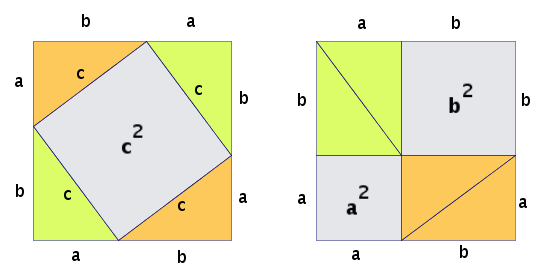
\includegraphics[width=\textwidth]{../img/pythagorus}

Write 1 page explaining this proof.
\end{frame}
\end{document}
